% Sandia National Laboratories is a multimission laboratory managed and
% operated by National Technology & Engineering Solutions of Sandia, LLC, a
% wholly owned subsidiary of Honeywell International Inc., for the U.S.
% Department of Energy’s National Nuclear Security Administration under
% contract DE-NA0003525.

% Copyright 2002-2020 National Technology & Engineering Solutions of Sandia,
% LLC (NTESS).


Semiconductor device simulation, which is based on a coupled set of partial
differential equations (PDE's) is supported in \Xyce{}.  Such devices can be
invoked from the circuit netlist in a manner similar to traditional SPICE-style
analog devices.  One dimensional and two dimensional devices are supported,
with the dimensionality determined by the device model level.

\begin{Device}

\item[1D Device Form]
\begin{alltt}
YPDE <name> <node> [node] [model name]
+ [device parameters]
\end{alltt}

\vbox{\hrulefill}
\item[2D Device Form]
\begin{alltt}
YPDE <name> <node> <node> [node][node] [model name]|
+ [device parameters]
\end{alltt}

\model
\begin{alltt}
.MODEL <model name> ZOD [model parameters]
\end{alltt}

\comments

All of the PDE parameters are specified on the instance level.  The model
statement is used only for specifying if the device is 1D or 2D, via the level
parameter.  Both the 1D and the 2D devices can construct evenly-spaced meshes
internally, or an unstructured mesh can be read in from an external mesh file.

The eletrode, doping and material parameters are specified using a special
format that is described in the tables that are referenced in the instance
parameter tables.
\end{Device}

\paragraph{TCAD Device Parameters}
Most TCAD device parameters are specified on the instance level.
\noindent
The only TCAD device model parameter is the level, which specifies whether the
model is one or two dimensions.

\label{PDE_Model_Params}
\index{PDE Devices!model parameters}
\begin{DeviceParamTable}{PDE Device Model Parameters}
LEVEL & Determines if the device is 1D or 2D  1=1D, 2=2D & -- & 1 \\ \hline
\end{DeviceParamTable}

\index{PDE Devices!1D instance parameters}
% This table was generated by Xyce:
%   Xyce -doc_cat Pde 1
%
\index{1d pde (level 1)!device instance parameters}
\begin{DeviceParamTableGenerated}{1D PDE (level 1) Device Instance Parameters}{Pde_1_Device_Instance_Params}
AUGER & Flag to turn on/off Auger recombination & logical (T/F) & true \\ \hline
BULKMATERIAL & Bulk semiconductor material & -- & 'SI' \\ \hline
DOPINGPROFILES &  & \multicolumn{2}{c}{See Table~\ref{DOPINGPROFILES_Composite_Params}}  \\ \hline
FERMIDIRAC & Use Fermi-Dirac statistics. & logical (T/F) & false \\ \hline
FIELDDEP & If true, use field dependent mobility. & logical (T/F) & false \\ \hline
LAYER &  & \multicolumn{2}{c}{See Table~\ref{LAYER_Composite_Params}}  \\ \hline
MASKVARSTIA & If set to true, then some variables are excluded from the time integration error control calculation. & logical (T/F) & false \\ \hline
MAXVOLTDELTA & Maximum voltage change used by two-level Newton algorithm. & V & 0.025 \\ \hline
MESHFILE &  & -- & 'internal.msh' \\ \hline
MOBMODEL & Mobility model. & -- & 'ARORA' \\ \hline
NODE &  & \multicolumn{2}{c}{See Table~\ref{NODE_Composite_Params}}  \\ \hline
NX & Number of mesh points & -- & 11 \\ \hline
REGION &  & \multicolumn{2}{c}{See Table~\ref{REGION_Composite_Params}}  \\ \hline
SRH & Flag to turn on/off Shockley-Read-Hall (SRH) recombination. & logical (T/F) & true \\ \hline
THERMIONICEMISSION &  & logical (T/F) & false \\ \hline
TUNNELING &  & -- & 'none' \\ \hline
USEOLDNI & Flag for using old(inaccurate) intrinsic carrier calculation. & logical (T/F) & false \\ \hline
VOLTLIM & Flag to apply voltage limiting.  This is only relevant for an experimental two-level Newton solver. & logical (T/F) & false \\ \hline

\category{Doping Parameters}\\ \hline
DOPING\_FILE & File containing doping profile. & -- & 'NOFILE' \\ \hline
GRADED & Flag for graded junction vs. abrupt junction. – (1/true=graded, 0/false=abrupt) & logical (T/F) & false \\ \hline
NA & Acceptor doping level & cm$^{-3}$ & 1e+15 \\ \hline
ND & Donor doping level & cm$^{-3}$ & 1e+15 \\ \hline
NDOPE\_FILE & File containing doping profile for N-type dopants. & -- & 'NOFILE' \\ \hline
PDOPE\_FILE & File containing doping profile for P-type dopants. & -- & 'NOFILE' \\ \hline
WJ & Junction width, if graded junction enabled. & cm & 0.0001 \\ \hline

\category{Geometry Parameters}\\ \hline
ANODE.AREA & Anode area (used for two-terminal devices) & cm$^{-2}$ & 0 \\ \hline
AREA & Cross sectional area of the device. & cm$^{-2}$ & 1 \\ \hline
BASE.AREA & Base area (used for three-terminal (BJT) devices) & cm$^{-2}$ & 0 \\ \hline
BASE.LOC & Location of base contact (necessary if running with three terminals). & cm & 0.0005 \\ \hline
CATHODE.AREA & Cathode area (used for two-terminal devices) & cm$^{-2}$ & 0 \\ \hline
COLLECTOR.AREA & Collector area (used for three-terminal (BJT) devices) & cm$^{-2}$ & 0 \\ \hline
EMITTER.AREA & Emitter area (used for three-terminal (BJT) devices) & cm$^{-2}$ & 0 \\ \hline
L & Device width. (Synonym with W parameter) & cm & 0.001 \\ \hline
W & Device width. (Synonym with L parameter) & cm & 0.001 \\ \hline

\category{Temperature Parameters}\\ \hline
TEMP & Device temperature & $^\circ$C & 27 \\ \hline

\category{Model Output Parameters}\\ \hline
FIRSTELECTRODEOFFSET & This is an output parameter.  It is only used if OFFSETOUTPUTVOLTAGE=true. (see description of that paramaeter & logical (T/F) & false \\ \hline
GNUPLOTLEVEL & Flag for gnuplot output.
0 - no gnuplot files.
1 - gnuplot files.
gnuplot is an open source plotting program that is usually installed on Linux systems. gnuplot files will have the *Gnu.dat suffix, and the prefix will be thename of the device instance. & -- & 1 \\ \hline
OFFSETOUTPUTVOLTAGE & This is an output parameter that determines the ``zero'' of the potential at output.  If OFFSETOUTPUTVOLTAGE=true (default) it will adjust the voltages at output so that the minimum voltage is zero. If true and also FIRSTELECTRODEOFFSET=true, then the voltage of the first electrode is the zero point.  If OFFSETOUTPUTVOLTAGE=false, the output voltage sets the intrisic Fermi level to zero.  Depending on circumstances each of these may be more or less convenient for plotting. & logical (T/F) & true \\ \hline
OUTPUTINTERVAL & Time interval for tecplot output (if tecplot is enabled). & s & 0 \\ \hline
OUTPUTNLPOISSON & Flag to determine if the results of the nonlinear Poisson calculation is included in the output files.  Normally, this calculation is used to initialize a drift-diffusion calculation and isn't of interest. & logical (T/F) & false \\ \hline
%SGPLOTLEVEL & Flag for sgplot output.
%0 - no sgplot files.
%1 - sgplot files.
%sgplot is a plotting program that comes as part of the SG Framework. sgplot files will have the *.res suffix, and the prefix will be the name of the device instance & -- & 0 \\ \hline
TECPLOTLEVEL & Setting for Tecplot output:
0 - no Tecplot files
1 - Tecplot files, each output in a separate file. 2 - Tecplot file, each outputappended to a single file.
Tecplot files will have the .dat suffix, and the prefix will be the name of the device instance & -- & 1 \\ \hline

\category{Scaling Parameters}\\ \hline
C0 & Density scalar; adjust to mitigate convergence problems.The model will do all of its scaling automatically, so it is generally not necessary to specify it manually. & cm$^{-3}$ & 1e+15 \\ \hline
DENSITYSCALARFRACTION & Fraction of the maximum doping by which density will be scaled.The model will do all of its scaling automatically, so it is generally not necessary to specify it manually. & logical (T/F) & 0.1 \\ \hline
SCALEDENSITYTOMAXDOPING & If set the density will be scaled by a fraction of the maximum doping.The model will do all of its scaling automatically, so it is generally not necessary to specify it manually. & logical (T/F) & true \\ \hline
t0 & Time scalar; adjust to mitigate convergence problems.The model will do all of its scaling automatically, so it is generally not necessary to specify it manually. & s & 1e-06 \\ \hline
X0 & Length scalar; adjust to mitigate convergence problems.The model will do all of its scaling automatically, so it is generally not necessary to specify it manually. & cm & 1e-07 \\ \hline

\category{Boundary Condition Parameters}\\ \hline
ANODE.BC & Anode voltage boundary condition.  Only used if device is uncoupled from circuit, and running in diode mode.
 & V & 0.5 \\ \hline
BASE.BC & Base voltage boundary condition.  Only used if device is uncoupled from circuit, and running in BJT mode.
 & V & 0 \\ \hline
CATHODE.BC & Cathode voltage boundary condition.  Only used if device is uncoupled from circuit, and running in diode mode.
 & V & 0 \\ \hline
COLLECTOR.BC & Collector voltage boundary condition.  Only used if device is uncoupled from circuit, and running in BJT mode.
 & V & 0 \\ \hline
EMITTER.BC & Emitter voltage boundary condition.  Only used if device is uncoupled from circuit, and running in BJT mode.
 & V & 0.5 \\ \hline
\end{DeviceParamTableGenerated}

\clearpage

\index{PDE Devices!1D instance parameters}
% This table was generated by Xyce:
%   Xyce -doc_cat Pde 2
%
\index{2d pde (level 2)!device instance parameters}
\begin{DeviceParamTableGenerated}{2D PDE (level 2) Device Instance Parameters}{Pde_2_Device_Instance_Params}
BULKMATERIAL & Material of bulk material. & -- & 'SI' \\ \hline
DISPLCUR & If true, displacement current is computed and output & logical (T/F) & false \\ \hline
DOPINGPROFILES &  & \multicolumn{2}{c}{See Table~\ref{DOPINGPROFILES_Composite_Params}}  \\ \hline
MAXVOLTDELTA & Maximum voltage change used by two-level Newton algorithm. & V & 0.025 \\ \hline
MESHFILE & This is a required field for a 2D simulation.  If the userspecifies meshfile=internal.mesh, the model will create aCartesian mesh using the parameters L,W,NX and NY.  If the user specifies anything else (for example meshfile=diode.msh), the model will attempt to read in a mesh file of that name.  The format is assumed to be that of the SG Framework. & -- & 'internal.msh' \\ \hline
MOBMODEL & Mobility model. & -- & 'ARORA' \\ \hline
NODE &  & \multicolumn{2}{c}{See Table~\ref{NODE_2D_Composite_Params}}  \\ \hline
NX & Number of mesh points, x-direction. & -- & 11 \\ \hline
NY & Number of mesh points, y-direction. & -- & 11 \\ \hline
REGION &  & \multicolumn{2}{c}{See Table~\ref{REGION_Composite_Params}}  \\ \hline
TYPE & P-type or N-type - this is only relevant if using the default dopings & -- & 'PNP' \\ \hline
USEMATRIXGID &  & -- & false \\ \hline
USEOLDNI & Flag for using old (inaccurate) intrinsic carrier calculation. & logical (T/F) & false \\ \hline
USEVECTORGID &  & -- & false \\ \hline
VOLTLIM &  & logical (T/F) & false \\ \hline

\category{Doping Parameters}\\ \hline
GRADED & Flag for graded junction vs. abrupt junction. – (1/true=graded, 0/false=abrupt) & logical (T/F) & false \\ \hline
NA & Acceptor doping level & cm$^{-3}$ & 1e+15 \\ \hline
ND & Donor doping level & cm$^{-3}$ & 1e+15 \\ \hline
WJ & Junction width, if graded junction enabled. & cm & 0.0001 \\ \hline

\category{Geometry Parameters}\\ \hline
AREA & Cross sectional area of the device. & cm$^{-2}$ & 1 \\ \hline
CYL & Flag to enable cylindrical geometry & logical (T/F) & false \\ \hline
L & Device length & cm & 0.001 \\ \hline
W & Device width & cm & 0.001 \\ \hline

\category{Temperature Parameters}\\ \hline
TEMP & Device temperature & $^\circ$C & 27 \\ \hline

\category{Model Output Parameters}\\ \hline
GNUPLOTLEVEL & Flag for gnuplot output.
0 - no gnuplot files.
1 - gnuplot files.
gnuplot is an open source plotting program that is usually installed on Linux systems. gnuplot files will have the *Gnu.dat suffix, and the prefix will be thename of the device instance. & -- & 0 \\ \hline
INTERPGRIDSIZE &  & -- & 20 \\ \hline
OUTPUTINTERVAL & Time interval for tecplot output (if tecplot is enabled). & s & 0 \\ \hline
OUTPUTNLPOISSON & Flag to determine if the results of the nonlinear Poisson calculation is included in the output files.  Normally, this calculation is used to initialize a drift-diffusion calculation and isn't of interest. & logical (T/F) & false \\ \hline
%SGPLOTLEVEL & Flag for sgplot output.
%0 - no sgplot files.
%1 - sgplot files.
%sgplot is a plotting program that comes as part of the SG Framework. sgplot files will have the *.res suffix, and the prefix will be the name of the device instance & -- & 0 \\ \hline
TECPLOTLEVEL & Setting for Tecplot output:
0 - no Tecplot files
1 - Tecplot files, each output in a separate file. 2 - Tecplot file, each outputappended to a single file.
Tecplot files will have the .dat suffix, and the prefix will be the name of the device instance & -- & 1 \\ \hline
TXTDATALEVEL & Flag for volume-averaged text output.
0 - no text files.
1 - text files.
txtdataplot files will have the *.txt suffix, and the prefix will be the name of the device instance. & -- & 1 \\ \hline

\category{Scaling Parameters}\\ \hline
X0 & Length scalar; adjust to mitigate convergence problems. The model will do all of its scaling automatically, so it is generally not necessary to specify it manually. & cm & 0.0001 \\ \hline

\category{Boundary Condition Parameters}\\ \hline
CONSTBOUNDARY &  & -- & false \\ \hline
\end{DeviceParamTableGenerated}

\clearpage

\paragraph{Layer Parameters}
% This table was generated by Xyce
\index{layer!composite parameters}
\begin{CompositeParamTableGenerated}{LAYER Composite Parameters}{LAYER_Composite_Params}
CON &  & -- & 1.42248 \\ \hline
ConductionBandDOS &  & -- & 2.89e+19 \\ \hline
DIEL &  & -- & 13.1 \\ \hline
ELMOB0 &  & -- & 2240 \\ \hline
ELVSAT &  & -- & 7.7e+06 \\ \hline
EMASS &  & -- & 0.067 \\ \hline
GRADEDWIDTH &  & -- & 0 \\ \hline
HMASS &  & -- & 0.5 \\ \hline
HOMOB0 &  & -- & 30 \\ \hline
HOVSAT &  & -- & 7.7e+06 \\ \hline
MATERIAL &  & -- & 'gaas' \\ \hline
NAME &  & -- & 'EMITTER' \\ \hline
NARCO &  & -- & 0.047 \\ \hline
NARVA &  & -- & 0.047 \\ \hline
NDOPE &  & -- & 0 \\ \hline
NI &  & -- & 1.79e+06 \\ \hline
NX &  & -- & 25 \\ \hline
PDOPE &  & -- & 5e+19 \\ \hline
VAL &  & -- & 0 \\ \hline
ValenceBandDOS &  & -- & 2.66e+19 \\ \hline
WIDTH &  & -- & 1e-06 \\ \hline
\end{CompositeParamTableGenerated}


\paragraph{Electrode Parameters 1D}
% This table was generated by Xyce
\index{node!composite parameters}
\begin{CompositeParamTableGenerated}{NODE Composite Parameters}{NODE_Composite_Params}
AREA &  & -- & 0 \\ \hline
BC & Carrier density boundary condition type (dirichlet or neumann) & -- & 'dirichlet' \\ \hline
LOCATION &  & -- & 0 \\ \hline
MATERIAL & Contact material & -- & 'neutral' \\ \hline
NAME & Electrode name & -- & 'anode' \\ \hline
OXIDEBNDRYFLAG & Oxide layer boolean & -- & false \\ \hline
SIDE & Side specification (left or right) & -- & 'left' \\ \hline
\end{CompositeParamTableGenerated}


\paragraph{Electrode Parameters 2D}
% This table was generated by Xyce
\index{node!composite parameters}
\begin{CompositeParamTableGenerated}{NODE Composite Parameters}{NODE_2D_Composite_Params}
BC & Carrier density boundary condition type (dirichlet or neumann) & -- & 'dirichlet' \\ \hline
END & Ending location & cm & 0 \\ \hline
MATERIAL & Contact material & -- & 'neutral' \\ \hline
NAME & Electrode name & -- & 'anode' \\ \hline
OXCHARGE & Oxide charge & -- & 0 \\ \hline
OXIDEBNDRYFLAG & Oxide layer boolean & -- & false \\ \hline
OXTHICK & Oxide thickness & cm & 0 \\ \hline
SIDE & Side specification (top, bottom, left or right) & -- & 'top' \\ \hline
START & Starting location & cm & 0 \\ \hline
\end{CompositeParamTableGenerated}


\paragraph{Doping or Region Parameters}
The \texttt{DOPINGPROFILES} and \texttt{REGION} parameters are synonyms,
therefore their tables of values are identical.  The use of both parameters in
the same device instance could lead to unpredictable behavior.
% This table was generated by Xyce
\index{dopingprofiles!composite parameters}
\begin{CompositeParamTableGenerated}{DOPINGPROFILES Composite Parameters}{DOPINGPROFILES_Composite_Params}
EL2 &  & -- & 0 \\ \hline
EXPRESSION & User-defined expressions for dopant profiles as function of depth  & -- & 'none' \\ \hline
FILE &  & -- & 'none' \\ \hline
FLATX & Determines the doping shape (half-gaussian or a full gaussian) & -- & 0 \\ \hline
FLATY & 2D ONLY: Determines the doping shape (half-gaussian or a full gaussian) & -- & 0 \\ \hline
FUNCTION & Functional form of doping region; options are uniform, gaussian, and step. & -- & 'uniform' \\ \hline
NAME &  & -- & 'none' \\ \hline
NMAX & Maximum value of impurity concentration & cm$^{-3}$ & 1e+15 \\ \hline
NMAXCHOP &  & cm$^{-3}$ & 1e+20 \\ \hline
NMIN & Minimum value of impurity concentration & cm$^{-3}$ & 0 \\ \hline
SPECIES &  & -- & 'none' \\ \hline
TYPE & ntype or ptype & -- & 'ntype' \\ \hline
XLOC & Peak location of the doping in the x-direction & cm & 0 \\ \hline
XMAX &  & cm & 0 \\ \hline
XMIN &  & cm & 0 \\ \hline
XWIDTH & Distance from nmax to nmin. This is only applicable for the function=gaussian case. & cm & 0.001 \\ \hline
YLOC & 2D ONLY: Peak location of the doping in the y-direction () & cm & 0 \\ \hline
YMAX & 2D ONLY:  & cm & 0 \\ \hline
YMIN & 2D ONLY:  & cm & 0 \\ \hline
YWIDTH & 2D ONLY: Distance from nmax to nmin. This is only applicable for the function=gaussian case. & cm & 0.001 \\ \hline
\end{CompositeParamTableGenerated}

% This table was generated by Xyce
\index{region!composite parameters}
\begin{CompositeParamTableGenerated}{REGION Composite Parameters}{REGION_Composite_Params}
EL2 &  & -- & 0 \\ \hline
EXPRESSION &  & -- & 'none' \\ \hline
FILE &  & -- & 'none' \\ \hline
FLATX & Determines the doping shape (half-gaussian or a full gaussian) & -- & 0 \\ \hline
FLATY & 2D ONLY: Determines the doping shape (half-gaussian or a full gaussian) & -- & 0 \\ \hline
FUNCTION & Functional form of doping region; options are uniform, gaussian, and step. & -- & 'uniform' \\ \hline
NAME &  & -- & 'none' \\ \hline
NMAX & Maximum value of impurity concentration & cm$^{-3}$ & 1e+15 \\ \hline
NMAXCHOP &  & cm$^{-3}$ & 1e+20 \\ \hline
NMIN & Minimum value of impurity concentration & cm$^{-3}$ & 0 \\ \hline
SPECIES &  & -- & 'none' \\ \hline
TYPE & ntype or ptype & -- & 'ntype' \\ \hline
XLOC & Peak location of the doping in the x-direction & cm & 0 \\ \hline
XMAX &  & cm & 0 \\ \hline
XMIN &  & cm & 0 \\ \hline
XWIDTH & Distance from nmax to nmin. This is only applicable for the function=gaussian case. & cm & 0.001 \\ \hline
YLOC & 2D ONLY: Peak location of the doping in the y-direction () & cm & 0 \\ \hline
YMAX & 2D ONLY:  & cm & 0 \\ \hline
YMIN & 2D ONLY:  & cm & 0 \\ \hline
YWIDTH & 2D ONLY: Distance from nmax to nmin. This is only applicable for the function=gaussian case. & cm & 0.001 \\ \hline
\end{CompositeParamTableGenerated}


\paragraph{Flat Parameters}
% Sandia National Laboratories is a multimission laboratory managed and
% operated by National Technology & Engineering Solutions of Sandia, LLC, a
% wholly owned subsidiary of Honeywell International Inc., for the U.S.
% Department of Energy’s National Nuclear Security Administration under
% contract DE-NA0003525.

% Copyright 2002-2021 National Technology & Engineering Solutions of Sandia,
% LLC (NTESS).


%%
%% Table describing the flatx, flaty parameters.
%%

\newenvironment{FlatTable}[1]
               {\renewcommand{\arraystretch}{1.5}
                 \newcommand{\category}[1]{\multicolumn{4}{c}{\smallskip\color{XyceDarkBlue}\em\bfseries ##1}}
                 \begin{longtable}{>{\ttfamily\small}m{1in}<{\normalfont}>{\raggedright\small}m{3in}>{\raggedright\let\\\tabularnewline\small}m{1in}}
                   \caption{#1} \\ \hline}
               {\end{longtable}}

%% ERK: Note:  I made each row of the table actually be two rows, because the 
%% graphical cross section picture, which is coming from a jpg file, was 
%% tending to overwrite the lines of the table.  In particular, it was 
%% overwriting the line immediately above it.  It did this for every 
%% (length, width) value that I tried.
%%
\begin{FlatTable}{Description of the flatx, flaty doping parameters\label{flatxy_table}}
    \rowcolor{XyceDarkBlue}
    \color{white}\normalfont\bf Flatx or Flaty view  &
    \color{white}\bf Description &
    \color{white}\bf 1D Cross Section \endhead

   0  & Gaussian on both sides of the peak (\texttt{xloc}) location. & {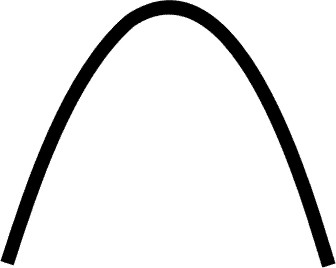
\includegraphics[width=0.300in,height= 0.300in]{flatxy1}} \\ \hline
  +1  & Gaussian if \texttt{x>xloc}, flat (constant at the peak value) if \texttt{x<xloc}. & {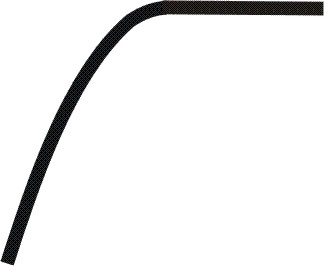
\includegraphics[width=0.300in,height= 0.300in]{flatxy2}} \\ \hline
  -1  & Gaussian if \texttt{x<xloc}, flat (constant at the peak value) if \texttt{x>xloc}. & {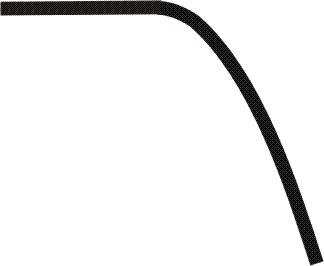
\includegraphics[width=0.300in,height= 0.300in]{flatxy3}} \\ \hline
\end{FlatTable}



